\documentclass[]{beamer}
\mode<presentation>
{
  \usetheme{Warsaw}
  \definecolor{mcgarnet}{rgb}{0.38, 0, 0.08}
  \definecolor{mcgray}{rgb}{0.6, 0.6, 0.6}
  \setbeamercolor{structure}{fg=mcgarnet,bg=mcgray}
  %\setbeamercovered{transparent}
}


\usepackage[english]{babel}
\usepackage[latin1]{inputenc}
\usepackage{times}
\usepackage[T1]{fontenc}
\usepackage{tikz}
\usepackage{graphicx}

\newcommand{\imagesource}[1]{{\centering\hfill\break\hbox{\scriptsize Image Source:\thinspace{\small\itshape #1}}\par}}

\title{12 - Strings and Objects}


\author{Dr. Robert Lowe\\}

\institute[Maryville College] % (optional, but mostly needed)
{
  Division of Mathematics and Computer Science\\
  Maryville College
}

\date[]{}
\subject{}

\pgfdeclareimage[height=0.5cm]{university-logo}{images/Maryville-College}
\logo{\pgfuseimage{university-logo}}



\AtBeginSection[]
{
  \begin{frame}<beamer>{Outline}
    \tableofcontents[currentsection]
  \end{frame}
}


\begin{document}

\begin{frame}
  \titlepage
\end{frame}

\begin{frame}{Outline}
  \tableofcontents
\end{frame}


% Structuring a talk is a difficult task and the following structure
% may not be suitable. Here are some rules that apply for this
% solution: 

% - Exactly two or three sections (other than the summary).
% - At *most* three subsections per section.
% - Talk about 30s to 2min per frame. So there should be between about
%   15 and 30 frames, all told.

% - A conference audience is likely to know very little of what you
%   are going to talk about. So *simplify*!
% - In a 20min talk, getting the main ideas across is hard
%   enough. Leave out details, even if it means being less precise than
%   you think necessary.
% - If you omit details that are vital to the proof/implementation,
%   just say so once. Everybody will be happy with that.

\section{Objects}

\begin{frame}{What is an object?}
    \begin{itemize}[<+(1)->]
        \item An \textbf{object} is an entity that has both state and
            behavior.
        \item It's a thing that ``remembers'' something and does
            something.
        \item In C++, objects allow us to have complex types with lots
            of useful abstract behavior.
    \end{itemize}
\end{frame}

\begin{frame}{The ``Black Box'' View of Objects}
\begin{columns}
    \column{0.6\textwidth}
    \begin{itemize}[<+->]
        \item When using objects, we think of them as ``black boxes''.
        \item The object does what it does, and we don't know or care
            how.
        \item Kind of like a soda machine.  
        \item By what arcane arts does the machine convert money into
            cold, bubbly, liquid candy?  
            \begin{itemize}
                \item Who knows?
                \item Who cares? (After we drink this stuff, the inner
                workings of the machine are the least of our worries!)
            \end{itemize}
    \end{itemize}

    \column{0.4\textwidth}
    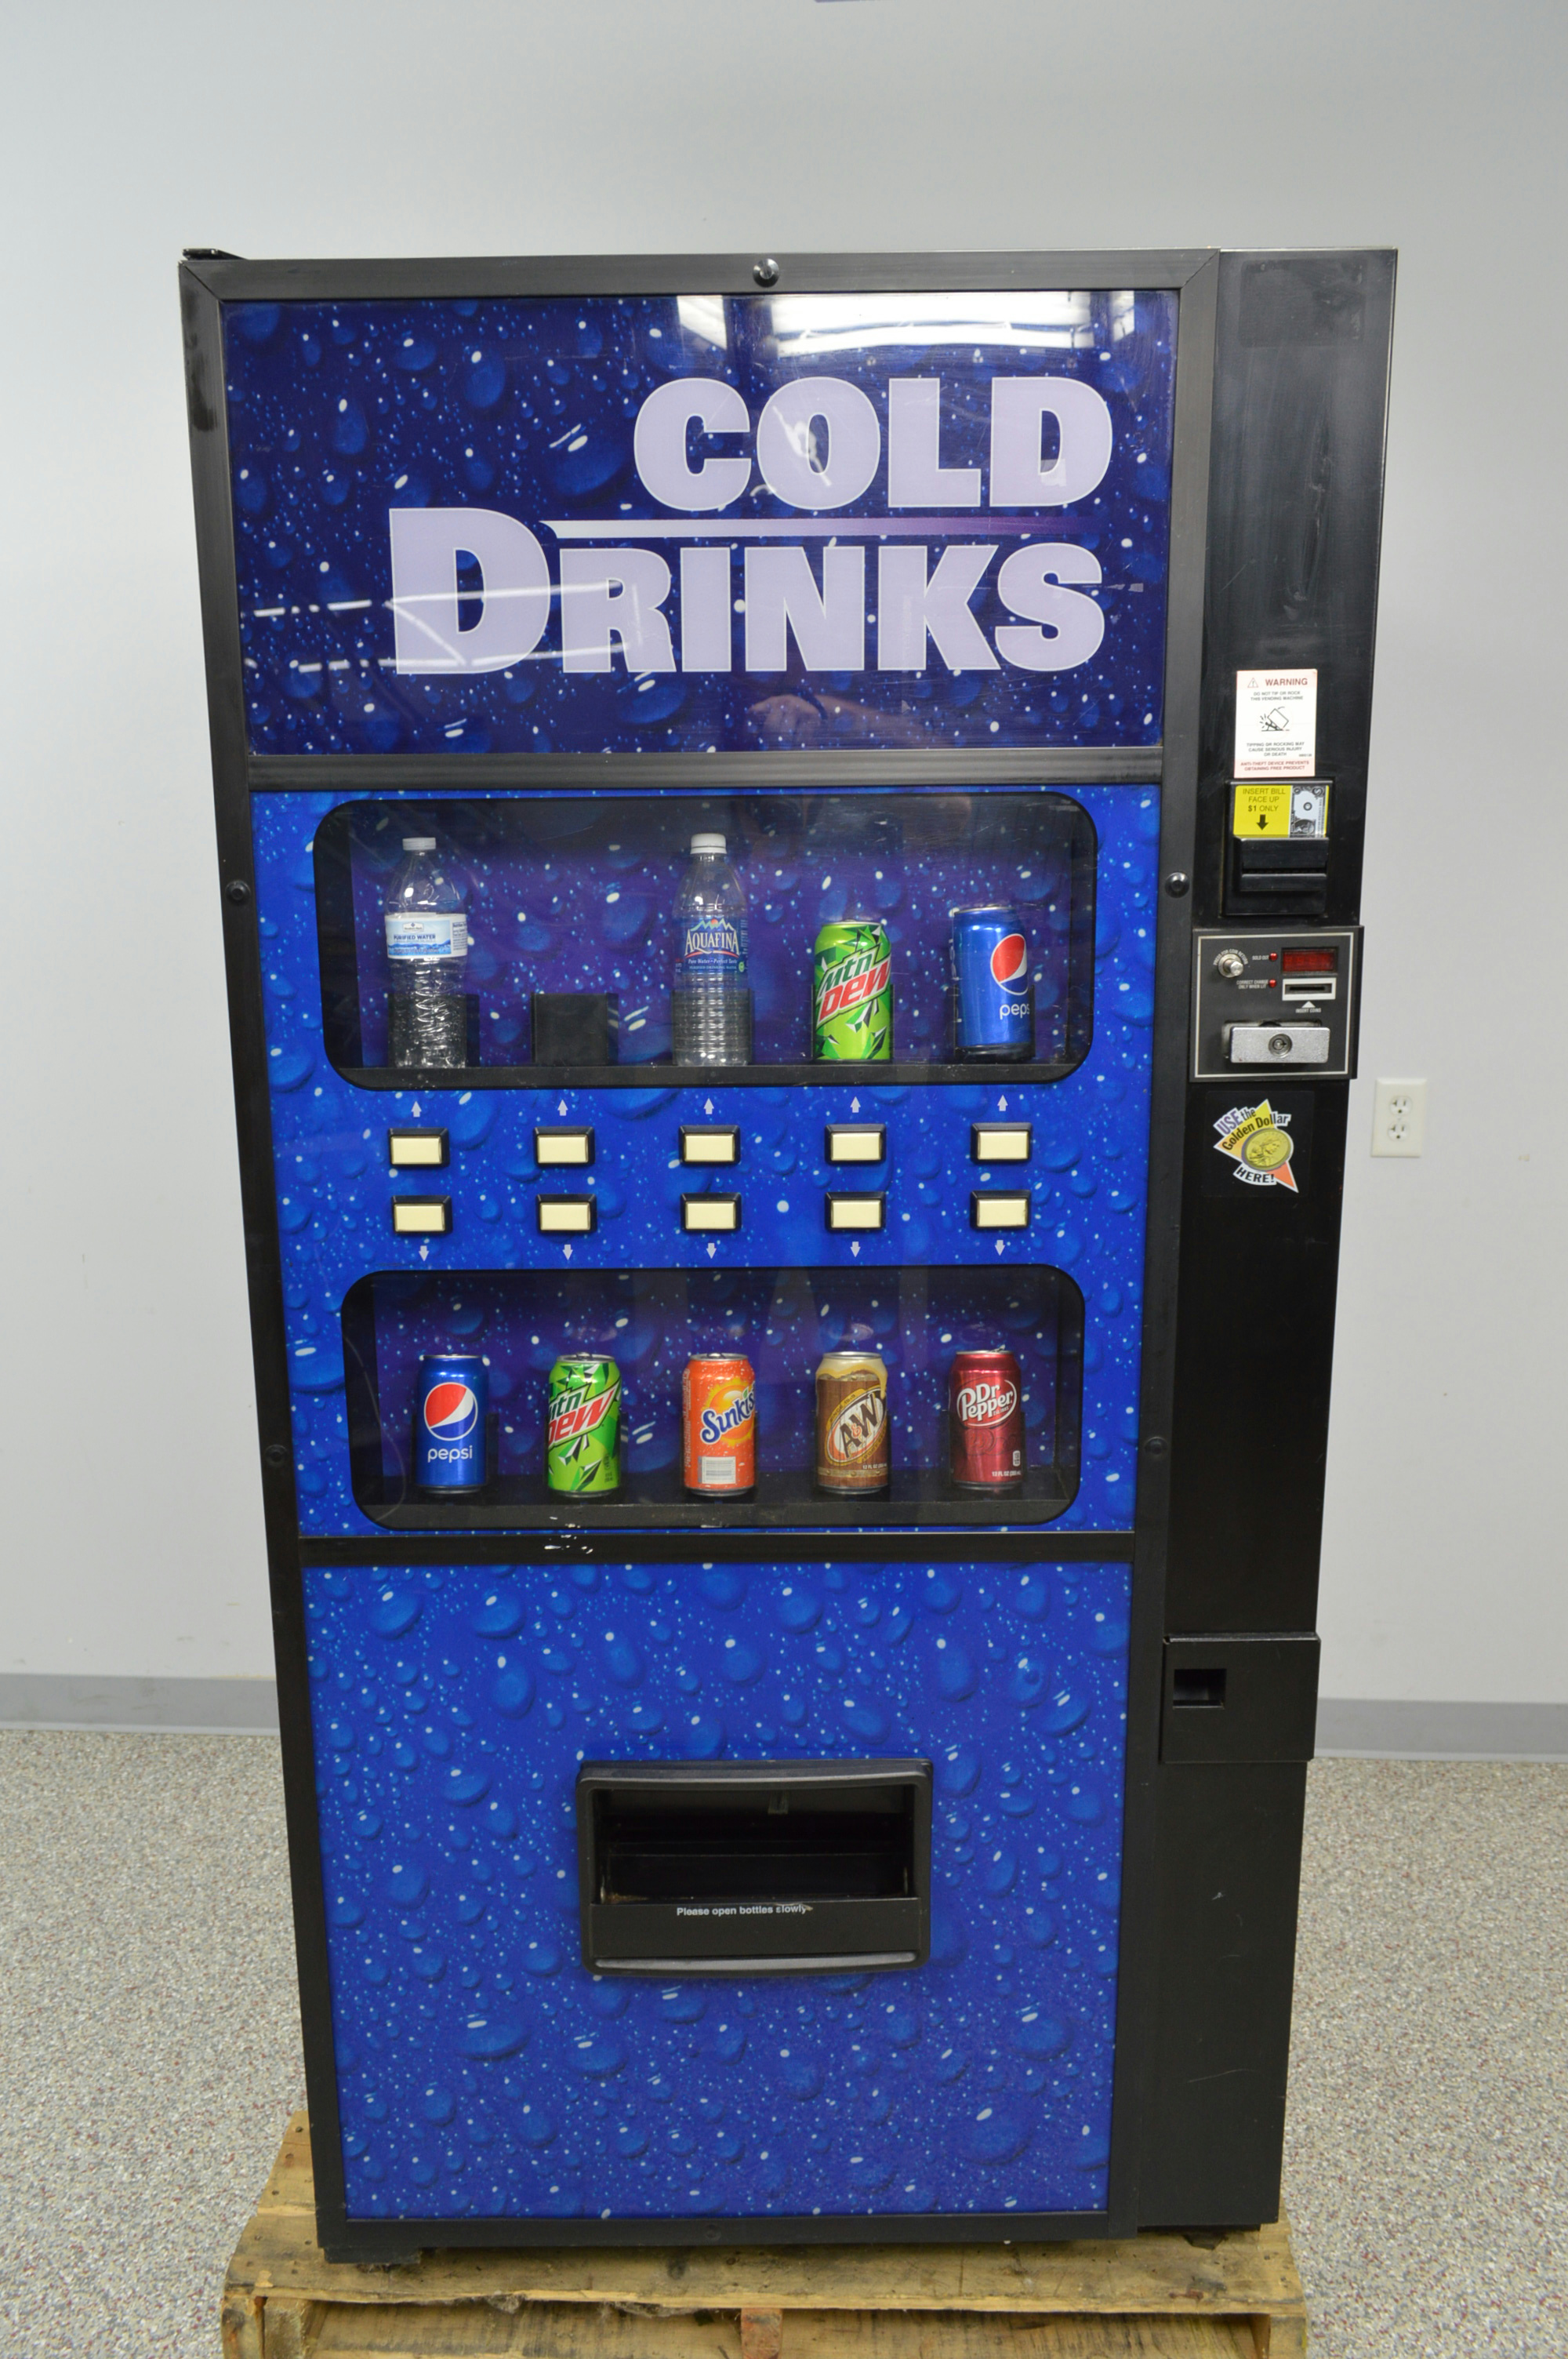
\includegraphics[width=\textwidth]{images/soda}
    {\tiny Image Source: \url{http://ebay.com}}
\end{columns}
\end{frame}


\begin{frame}{Accessing Object Functions}   
    \begin{itemize}[<+->]
        \item Every object is a scope unto itself.
        \item Every object contains member functions or
            \textbf{methods}.
        \item Every object also contains member variables.
        \item The member methods operate on the member variables.
        \item We access members by using the ``\texttt{.}'' operator.
        \item For example, suppose we had an object \texttt{str} which
            has a method \texttt{length}.  We would call this method
            like so:
            \newline\texttt{str.length();}
    \end{itemize}
\end{frame}

\begin{frame}{Objects Types}
    \begin{itemize}[<+->]
        \item Like everything else in C++, objects have types.
        \item In C++, an object's type is its \textbf{class}.
        \item The class of an object determines what member methods
            and variables it has.
        \item Later on, we will define our own classes.  For now, we
            will simply make use of pre-existing classes.
    \end{itemize}
\end{frame}


\section{Strings}

\begin{frame}{String Literals and C-Strings}
    \begin{itemize}[<+->]
        \item Recall that a string literal has quotation marks around
            it.  Example: \texttt{``Hello, world''}.
        \item The actual type of this literal is \texttt{const char[]}.
        \item That is, an array of constant characters.  
        \item This is a sequence of characters stored in contiguous
            memory:
            
            \begin{tabular}{|c|c|c|c|c|c|c|c|c|c|c|c|c|}
            \hline
            \texttt{H} & \texttt{e} & \texttt{l} & \texttt{l} & \texttt{o}
            & \texttt{,} & \texttt{ } & \texttt{W} & \texttt{o}
            & \texttt{r} & \texttt{l} & \texttt{d}& $\emptyset$ \\ 
            \hline
            \end{tabular}

        \item C-Strings can be difficult to work with.
        \item They cannot grow or shrink, and literal strings are
            immutable.
        \item Fortunately, C++ gives us a better way!
    \end{itemize}
\end{frame}

\begin{frame}{C++ Strings}
    \begin{itemize}[<+->]
        \item C++ provides a string object which abstracts away the
            details of how stings work.
        \item To use the string objects, you need to include the
            string header:
            \newline\texttt{\#include <string>}
        \item String objects are declared with the class type
            \texttt{string}: \newline\texttt{string str;}
        \item String objects can also be assigned string literal:
            \newline\texttt{str = "Hello, world";}
        \item C++ strings can grow and shrink as needed. They are much
            more convenient than C strings!
    \end{itemize}
\end{frame}


\begin{frame}{String Demonstration}
    \begin{itemize}[<+->]
        \item Go ahead and compile and and run
          \texttt{examples/12-Strings/string\_demo.cpp}
        \item First we have the \texttt{string} declaration and
            initialization:
            \newline\texttt{string str = "Hello, World";}
        \item Then we can see that strings interact with output
            streams:
            \newline\texttt{cout << "The string is: " << str << endl;}
        \item Another handy method allows us to get the length of
            a string:
            \newline\texttt{str.length()}
    \end{itemize}
\end{frame}

\begin{frame}[fragile]{Indexing Characters}

    \begin{tabular}{|r|c|c|c|c|c|c|c|c|c|c|c|c|}
    \hline
    \textbf{Character} & \texttt{H} & \texttt{e} & \texttt{l} & \texttt{l} & \texttt{o} & \texttt{,} & \texttt{ } & \texttt{W} & \texttt{o} & \texttt{r} & \texttt{l} & \texttt{d} \\ 
    \hline 
    \textbf{Index} & 0 & 1 & 2 & 3 & 4 & 5 & 6 & 7 & 8 & 9 & 10 & 11 \\ 
    \hline
    \end{tabular}

    \begin{itemize}[<+->]
        \item Each character in a string occupies a numbered slot.
        \item The number of each position is called an \textbf{index}.
        \item In C++, indexes (alas) begin at zero.
        \item The largest index in a string will be its
            \texttt{length() - 1}
        \item Hence the following loops through every index in the
            string:
\begin{verbatim}
//Loop over each character in the string
for(int i=0; i<str.length(); i++) {
    cout << i << ": " << str[i] << endl;
}
\end{verbatim}
        \item Note the use of the index operator \texttt{[]}.
        \item Discuss: Why must an index be an integer? 
    \end{itemize}
\end{frame}

\begin{frame}{Substrings}
    \begin{itemize}[<+->]
        \item Another handy feature of strings is the ability extract
            substrings.
        \item A \textbf{substring} is a segment within a larger
            string.
        \item The \texttt{substr} function has two versions:
            \begin{itemize}
                \item \texttt{substr(start)}
                \item \texttt{substr(start, len)}
            \end{itemize}
        \item Both are demonstrated in \texttt{string\_demo.cpp}.
            What do they each do?
    \end{itemize}
\end{frame}

\begin{frame}{Strings and Extraction Operators}
    \begin{itemize}[<+->]
        \item Take a look at \texttt{examples/12-Strings/name.cpp}
        \item Run the program.  What can you say about the extraction
            operator and strings?
        \item When you run the extraction operator, it only reads
            until the next space!
    \end{itemize}
\end{frame}

\begin{frame}{The \texttt{getline} Function}
    \begin{itemize}[<+->]
        \item The \texttt{getline} function allows us to read an
            entire line of text into a string.
        \item Its function prototype is:
            \newline\texttt{getline(istream \&is, string \&str);}
        \item Make a new directory: \texttt{labs/week8}
        \item Copy \texttt{name.cpp} into \texttt{labs/week8}
        \item Change the input line to the following:
            \newline\texttt{getline(cin, name);}
        \item Discuss:  Why isn't getline a member of string?
    \end{itemize}
\end{frame}

\begin{frame}{Lab Activity: Palindrome Detector}
    \begin{itemize}[<+->]
        \item A palindrome is a string that reads the same backwards
            and forwards.  
        \item For instance ``racecar'' is a palindrome.
        \item Let's design and implement a program which reads in
            a line of text and then determines if it is a palindrome
            or not!
        \item Now, let's make our palindrome program ignore the
            following:
            \begin{itemize}
                \item Ignore Case
                \item Ignore Punctuation
                \item Ignore Spaces
            \end{itemize}
    \end{itemize}
\end{frame}

\begin{frame}{The \texttt{cctype} Library}
    \begin{itemize}[<+->]
        \item The cctype library (\texttt{\#include<cctype>}) contains
            lots of handy functions to help us deal with characters.
            Some of these that may come in handy are:
            \begin{itemize}
                \item \texttt{toupper(c)}
                \item \texttt{tolower(c)}
                \item \texttt{isalpha(c)}
                \item \texttt{isspace(c)}
            \end{itemize}
        \item Let's finish the palindromes!
    \end{itemize}
\end{frame}

\end{document}


